\def\year{2015}

%File: formatting-instruction.tex
\documentclass[letterpaper]{article}
\usepackage{aaai}
\usepackage{times}
\usepackage{helvet}
\usepackage{courier}
%%
\usepackage{graphicx}
\usepackage{url}
\usepackage{amsfonts}
\usepackage{moreverb}
%%
\usepackage{bm}
\usepackage{paralist}
%\usepackage{minted}
%%
% so we don't need to specify figures subdirectory in figure code
\graphicspath{{./figures/}}
\usepackage{subfig}
%needed to change table colors
\usepackage[table]{xcolor}
\renewcommand{\arraystretch}{1.2} % General space between rows (1 standard)

%%
\frenchspacing
\setlength{\pdfpagewidth}{8.5in}
\setlength{\pdfpageheight}{11in}
\pdfinfo{
/Title (Insert Your Title Here)
/Author (Put All Your Authors Here, Separated by Commas)}
\setcounter{secnumdepth}{0}  
 \begin{document}
 \begin{sloppy}
% The file aaai.sty is the style file for AAAI Press 
% proceedings, working notes, and technical reports.
%
\title{Activity Monitoring and Prediction for Humans and NAO Humanoid Robots using 
Wearable Sensors}
\author{Saminda Abeyruwan \and Faisal Sikder \and Ubbo Visser \and Dilip Sarkar\\
 University of Miami \\
Department of Computer Science\\
 1365 Memorial Drive, Coral Gables, FL, 33146, USA\\
{\ttfamily \{saminda|f.sikder|visser|sarkar\}@cs.miami.edu}
}
\maketitle
\begin{abstract}
\begin{quote}
While humans or biped humanoid robots perform normal activities such as jogging, running and so 
on, an abnormal event such as a fall may occur. These events may cause damage to the human body or 
to the structural components of the humanoid robot. For humans, immediate identification of a fall 
will allow fast responses, while for a robot, early prediction can be used to take corrective 
measures to prevent a fall. There are inexpensive wireless sensing devices which can be  attached 
to humans or robots for collecting motion data. This paper unifies: \begin{inparaenum}[1)] \item 
methods to learn and predict different activities for humans and robots; and \item software 
tools to realize these functions  on embedded devices. \end{inparaenum} Our contributions include: 
\begin{inparaenum}[1)] \item detection of falls for both humans and robots within a unified 
framework; and \item  a  novel software development environment for embedded systems. 
\end{inparaenum} Our empirical evaluations demonstrate that with high accuracy different types of  
fall-events are predicted using the same learning algorithms for humans and biped humanoid robots. 
\end{quote}
\end{abstract}

\section{Introduction}
\label{sec:Intro}
The humans as well as the biped humanoid robots complete apparently simple activities that requires 
complex computational tasks such as jogging, running and so on. While performing these safe 
activities, accidents such as falls may occur causing damage to the human body or to the structural 
components of the humanoid robot \cite{li2009accurate}. There has been an increasing demand in 
domains such as rescue to use autonomous or teleoperated humanoid robots to complete high-risk 
tasks, otherwise would have been lethal to a human subject. Therefore, we envision environments 
where humans and humanoid robots collaboratively work to complete tasks. 

Since both humans and biped humanoid robots have almost identical movements and are susceptible to 
similar accidents, we believe that the same set of learning algorithms are suitable for both 
groups. In this paper,  to validate our hypotheses, we develop a generalize approach for learning 
and predicting activities of both groups.  We have attached wearable sensing devices to collect 
motion data and have used software tools to interpret the sensor data to distinguish 
between normal and abnormal activities. The sensing devices are assembled using off-the-shelf 
hardware component boards and the generalize software tools are developed by ourselves to 
collect data for learning and predicting activities. The software tools provide a modular 
functionalities to use for collecting  data from any sensing devices, and to learn and predict 
on/off-line. While attempts for identifying human motions have already been investigated, to the 
best of our knowledge, we are the first to investigate the prospect of using external embedded 
devices to identify activities on a NAO humanoid robot. Before we report our contributions, we 
provide a brief review of work related to identification of human activity.  


\subsection{Related Work}

The modern activity detection methods can be broadly categorized in to two groups based on: 
\begin{inparaenum}[1)] \item inexpensive wearable embedded devices; and \item smart-phones. 
\end{inparaenum} Wearable embedded devices with add-on sensors provide options to develop effective 
activity recognition methods for humans and biped humanoid robots alike. The existing activity 
detection methods focus on special cases of fall detection in humans and humanoid robots. These 
methods were primarily used in isolation.  {~\cite{ojetola2011fall}} reported method using 
accelerometers and gyroscopes to detect fall incidence among the elderly people. The work reported 
detecting four falling events: forward, backward, right, and left.  They used a decision tree to 
learn and classify falls and activities of daily living (ADL). The method identified fall events 
with precision of 81\%  and recall of 92\%. 

\cite{baek2013real} proposed  a fall  detection  system  using necklace-shaped tri-axial
accelerometer  and  gyroscope  sensors  to  classify  the  behavior  and  posture  of  the detection
 subject. Their method distinguished between  ADL and  fall, with  sensitivities  greater  than 
 80\%  and specificities  of  100\%. They experimented with ADLs such as: standing, sitting in the 
 chair or floor, laying, walking, running, going upstairs/downstairs, and bending, while, 
 falling forward, backward, leftward, rightward, and fall on the stairs were treated as abnormal 
 events. 
 
\cite{leone2013supervised} prosed a system to detect event that cause trauma, and disabilities
using a tri-axial MEMS wearable wireless accelerometer. They used support vector machine (SVM) for
robust classification of different events. \cite{Bao04activityrecognition} reported of using five 
small biaxial wire-free accelerometers attached  on the left bicep, right wrist, left quadriceps, 
right ankle, and right hip to recognize 20 activities starting from  walking  to  riding elevator  
to  strength  training to bicycling. They reported using decision table, instance-based learning, 
decision tree, and na\"{i}ve Bayes classifiers, where, decision tree showed the best performance 
with 84\% accuracy.  Similar efforts have been reported to detect human motions using motion 
tracking, e.g., 
\cite{dumitrache2013fall,kumarwearable,krishnan2014activity,gao2014evaluation,alvarez2015evaluating}.
 


{~\cite{moya2014fall}} proposed a fall detection, avoidance, and damage 
reduction mechanism for biped humanoid robots. They tried to simulate the real world environment 
where humanoid robots have to walk over irregular surface, running or playing sports, collusion 
with other robots. Their framework detected instability and did fall avoidance or at 
least low-damage falling mechanism was invoked. Therefore, embedded devices  with add-on sensors 
provide a flexible platform to build may real world applications. 


There is an increasing popularity in using smart-phones to detect activities in health care domain. 
Using only the accelerometer readings from a smart-phone, \cite{bai2013recognition} analyzed five 
actions of human walking, running, standing up, sitting down, and jumping. They compared the 
acceleration characteristics of these actions with three different fall accelerations to infer the 
direction of the fall. Their method recognize the fall activity, only when a predefined set of 
conditions were met. But the method did not provide any prediction or indication value, that a fall 
may occur in future. 

\cite{steidl2012fall} reported that the sensors of the smart-phones from different manufactures 
record values significantly incompatible ranges for identical tasks. Therefore, they trained a SVM 
classifier based on the features extracted from raw accelerometer readings and the directional 
changes of the constraining force exerted on an accelerometer to detect fall events. They compared 
these events to non-fall activities such as walking, running, jumping, and some actives which 
resembles falls such as sitting down on a chair. Their method detected fall events 84.8\% average 
accuracy across different smart-phones. 

\cite{DernbachDKTC12} explored methods to detect simple and complex activities using inertial 
sensors (accelerometer and gyroscope) of an Android smart-phone. The simple activities included: 
biking, climbing stairs, driving, running, sitting, standing, walking, and state of the phone not 
on the person. The complex activities were: cleaning, cooking, medication, sweeping, washing hands, 
and watering plants. Six different classifiers, multi-layer  perceptron (MLP), na\"{i}ve  Bayes,  
Bayesian  network,  decision  table,  best-first tree, and  K-star,  were trained on using the same 
feature extractor. For simple activities, 93\% accuracy using MLP were reported, while, 50\% 
success was achieved for complex activities.     


Similar to exiting methods, we have defined different normal and abnormal activities for humans and 
NAO humanoid robots. In order to validate our hypotheses that the learning and predicting methods 
unifies across the two groups, firstly, we have restricted the activities that can be performed 
on a NAO robot. Therefore, in our experiments, the human performed activities that are similar to 
robot, such as, walk or falling forward/backward so forth. Secondly, we have extended the human 
activities to a more complex events.  We have used Texas Instruments 
(TIs)\footnote{\url{https://www.ti.com/}}  microcontrollers and boosterpacks for our experiments, 
but, one can use microcontrollers and 
 sensor boards from other sources.  


%  The microcontrollers and embedded devices provide a flexible platform to build may 
% real world applications. In order to build these applications, a practitioner would require  
% flexible and reliable software solutions. A practitioner also may require to use more than one 
% functionality provided by the devices to build applications. Existing software solutions provide 
% facilities to build applications to a certain degree, but, they lack methods or systems to 
% integrate 
% multiple devices simultaneously without much user burden. We have developed  a state-of-the-art 
% open 
% source software solution to build heterogeneous applications on many devices, which can be 
% programmed on multiple operating systems. 

\begin{figure*}[!t]
\centering
\subfloat[]{\label{fig:fa}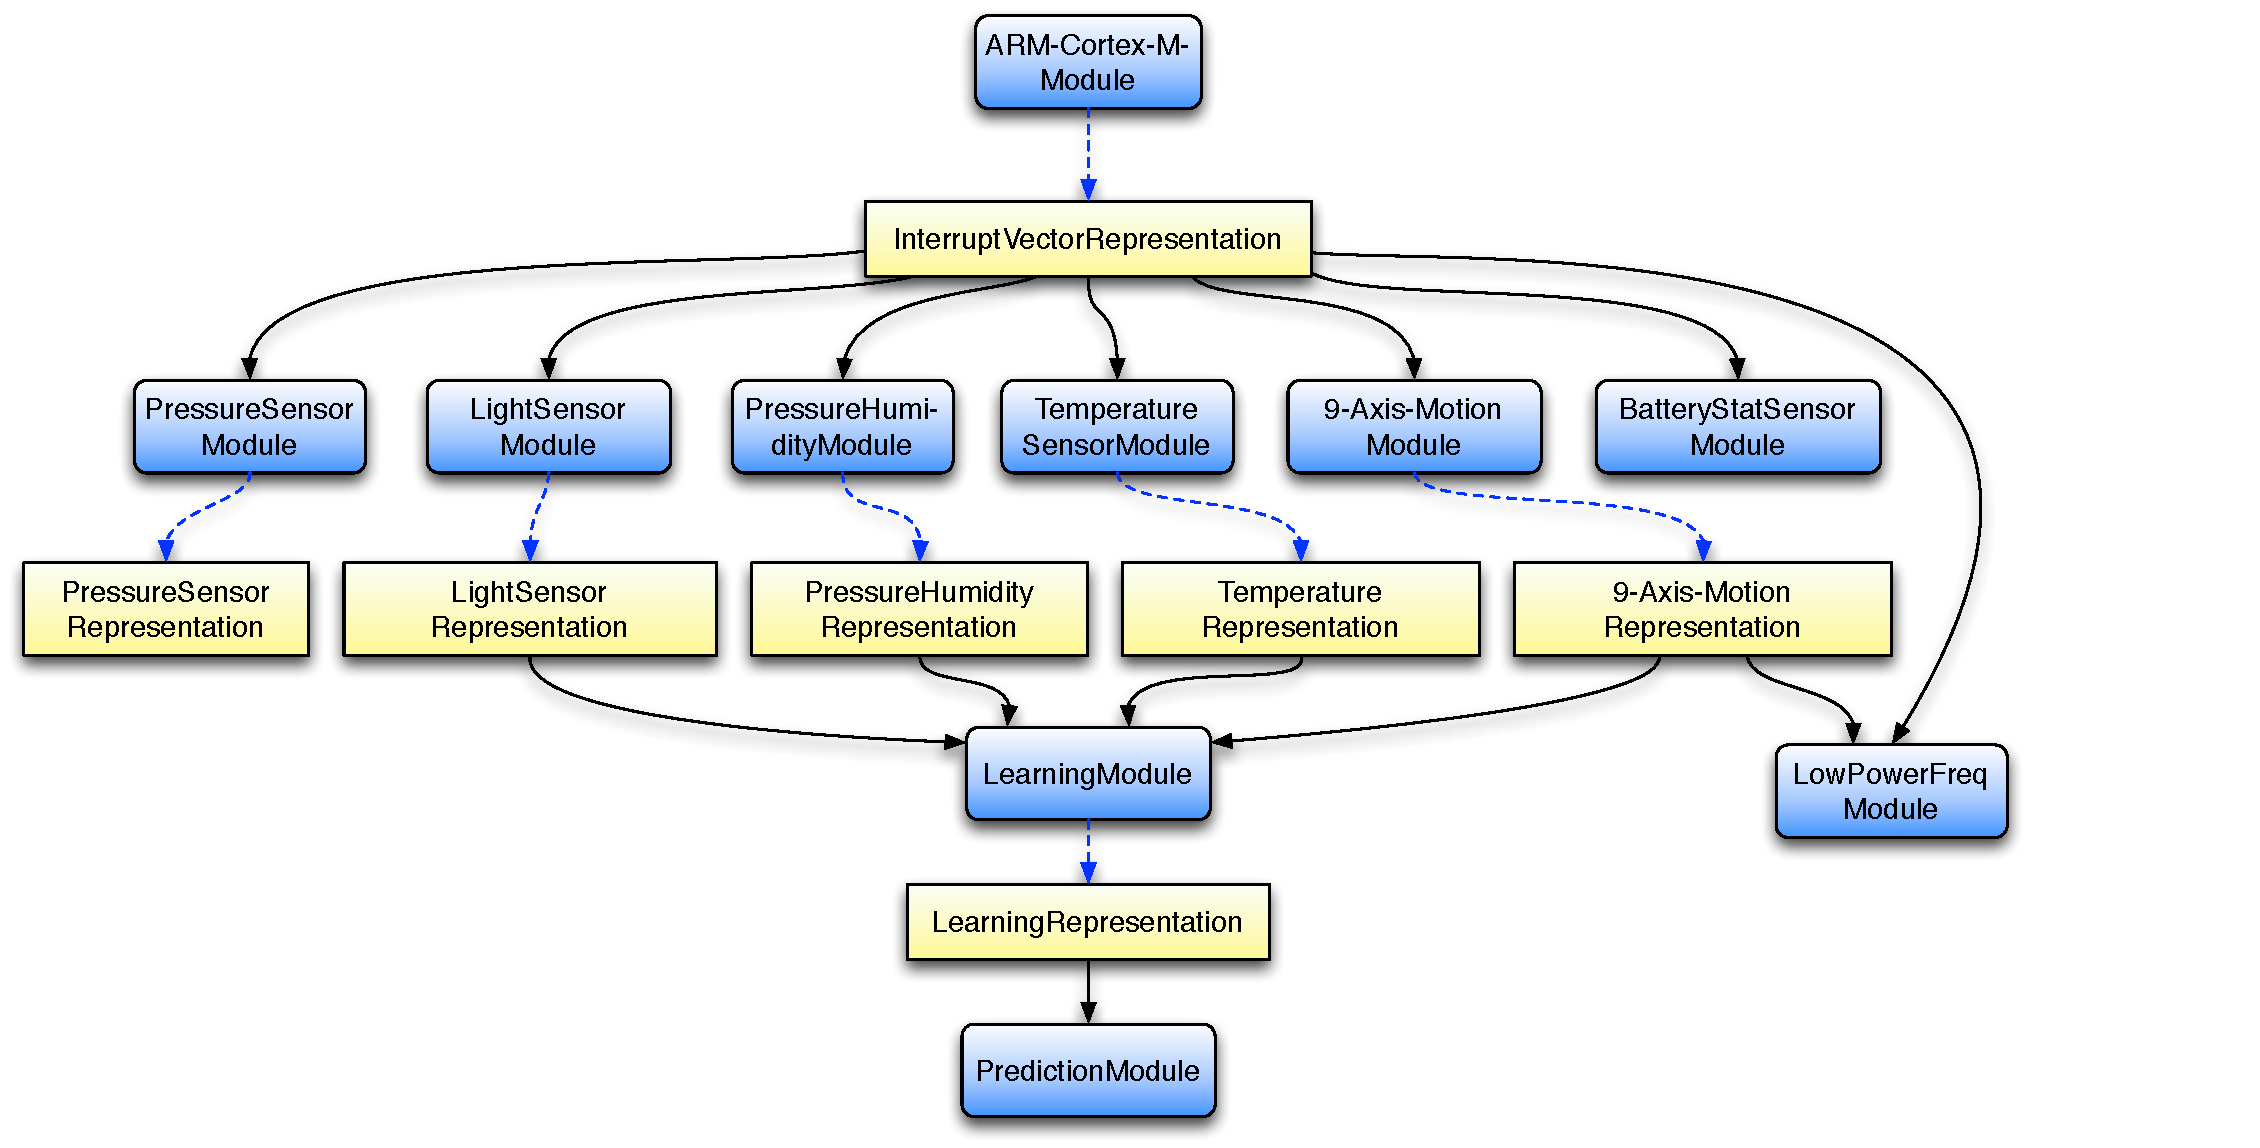
\includegraphics[width=0.6\textwidth]{figures/graph_structure_def-crop3}}
\subfloat[]{\label{fig:fb}\includegraphics[width=0.21\textwidth]{figures/human_figure}}
\subfloat[]{\label{fig:fc}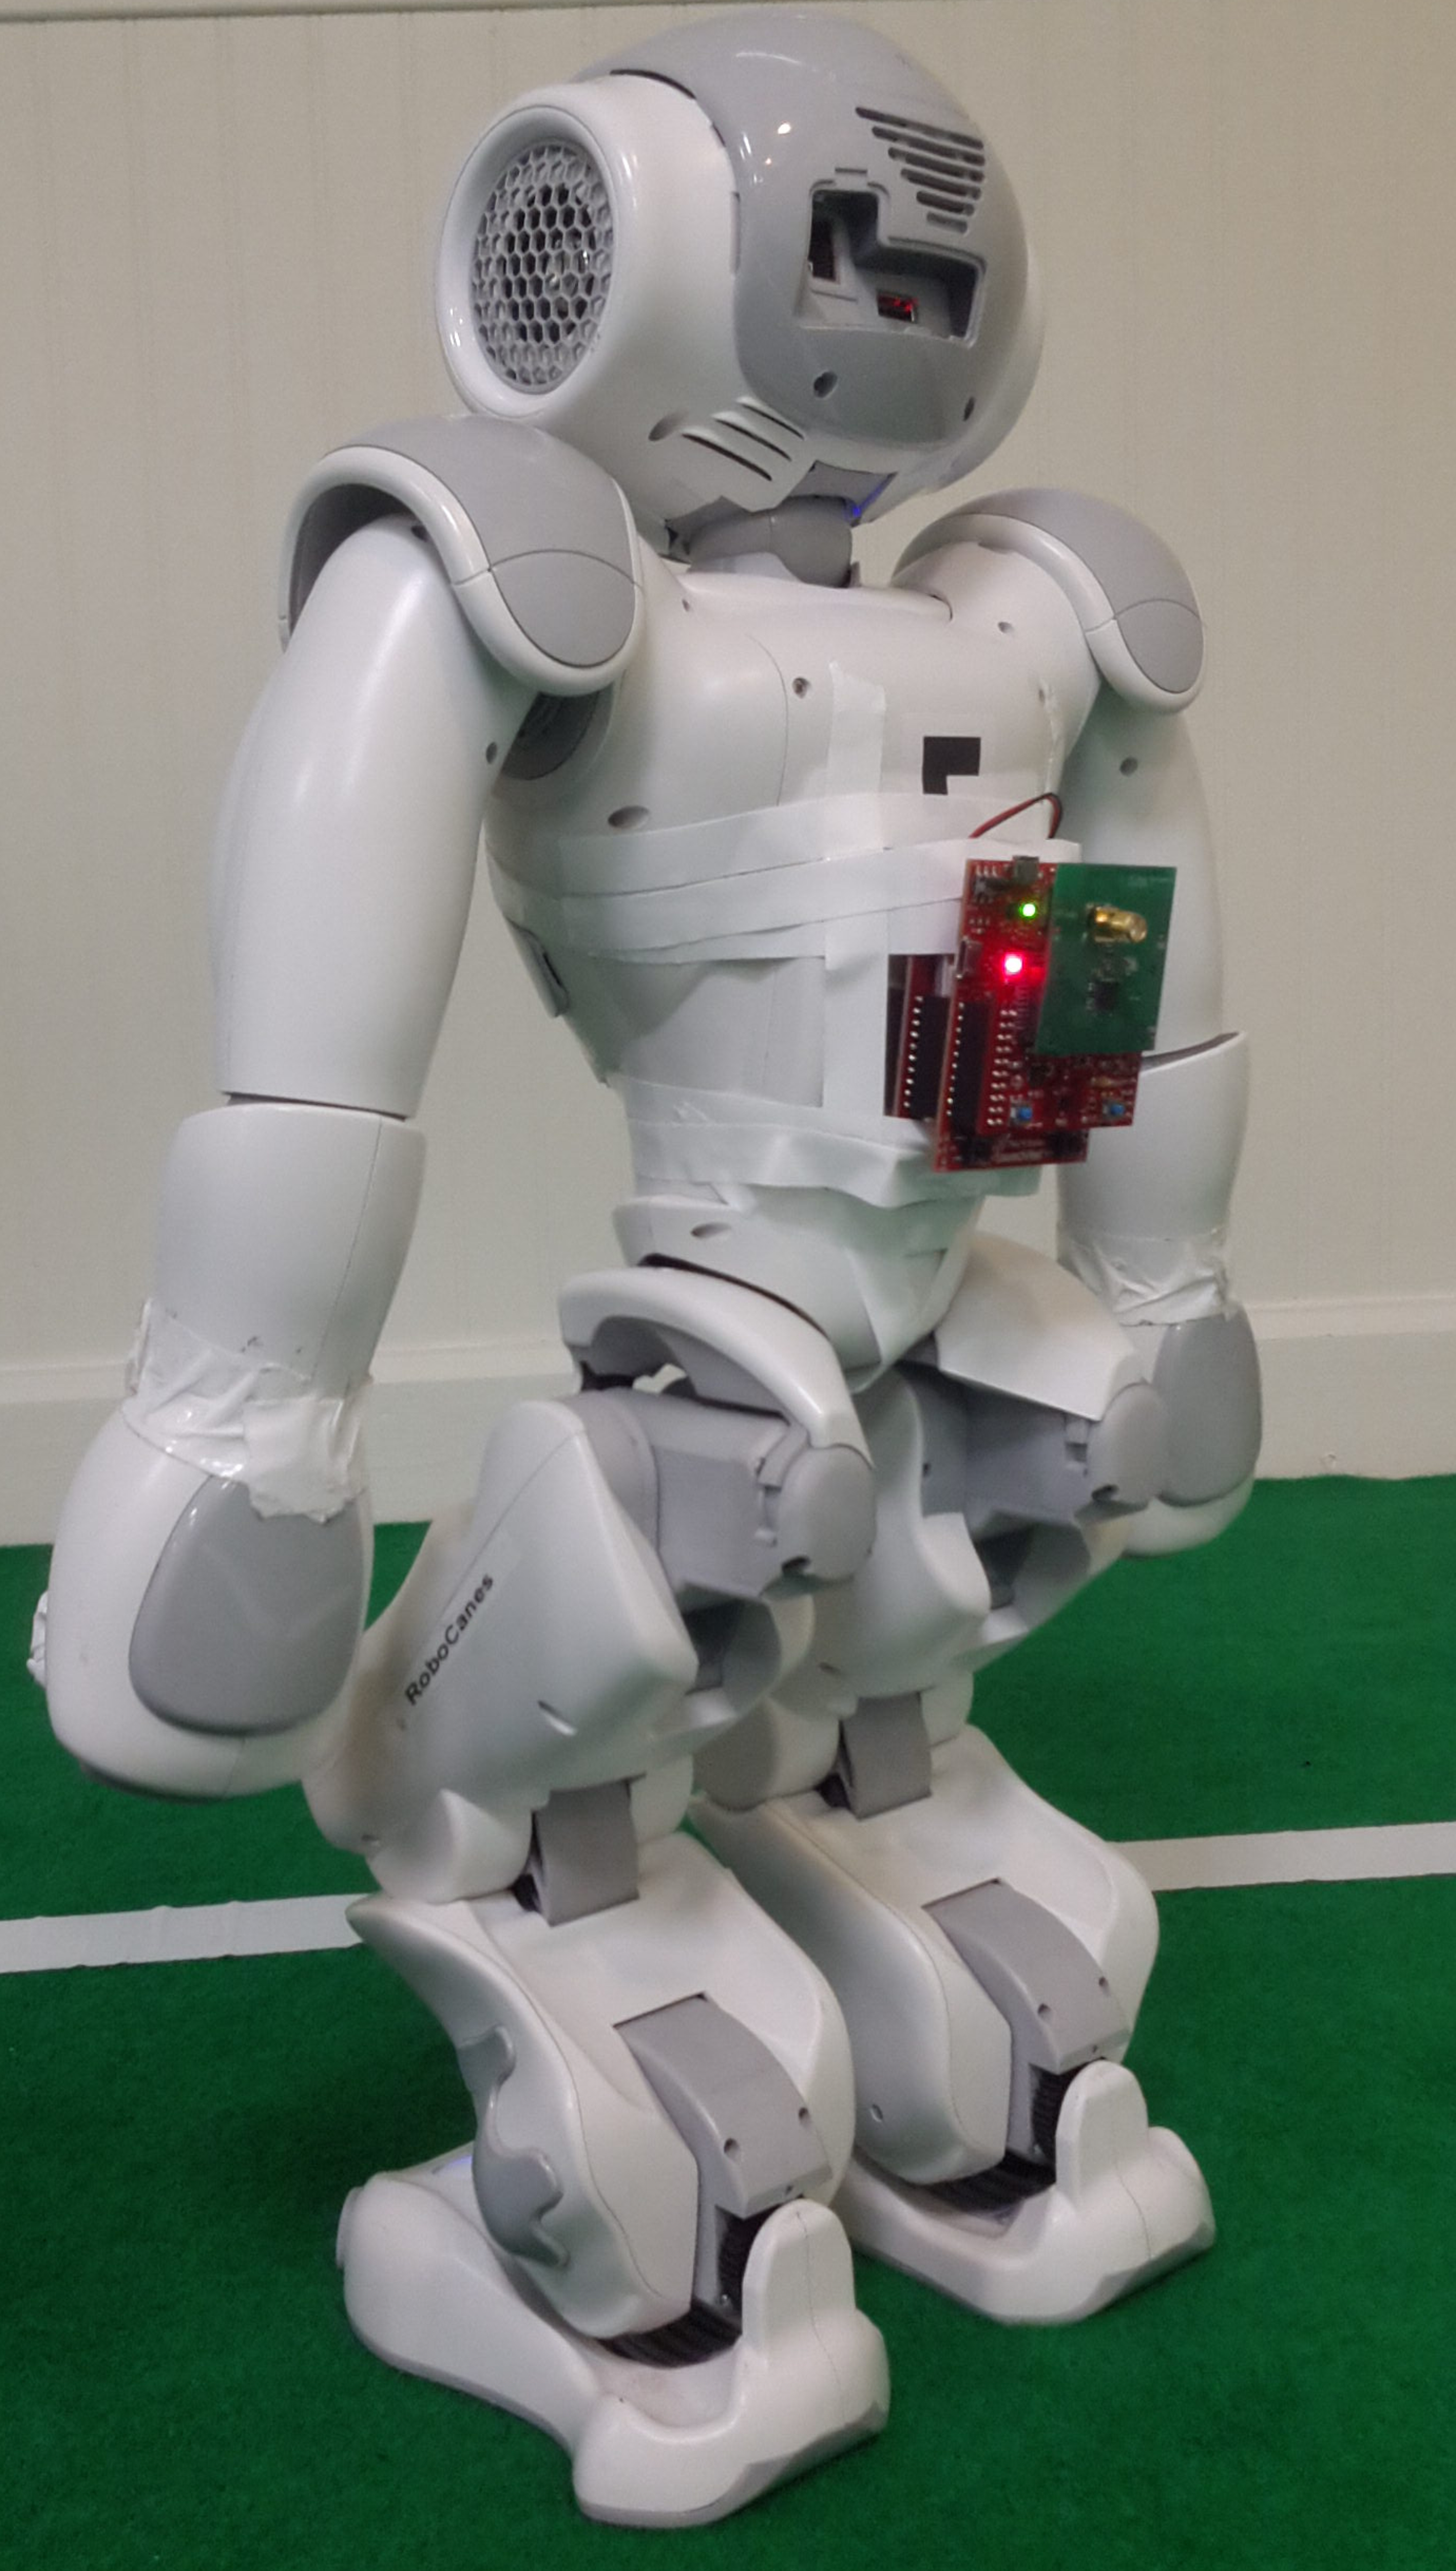
\includegraphics[width=0.185\textwidth]{figures/robot_figure}} 
\caption{(a) The modules and representations used in the experiments;  (b) the wireless transmitter 
was attached to a Sensor Hub BoosterPack on a Tiva C LaunchPad microcontroller that was connected 
to a Fuel Tank BoosterPack, which was then attached to the back of a human subject; and (c) the 
same device configuration was used on the back of a NAO humanoid robot.}
 \label{fig:framework}
\end{figure*}

\subsection{Our Approach and Contributions}

TI microcontrollers  boards such as MSP430{\texttrademark}LaunchPad, Tiva{\texttrademark} C Series 
TM4C123G LaunchPad, Tiva C Series TM4C129 Connected LaunchPad, and add-on booster packs such as 
Sensor Hub BoosterPack and CC2533  wireless transmitter and receiver  provide flexible platform for 
developing solutions for a wide rage of low power and portable applications. For our experiments, 
we have assembled a device with Tiva C Series TM4C123G microcontroller board, and three 
boosterpacks. The boosterpacks are for sensing 9-axis motion, battery power, and wireless 
networking. We have used two of the assembled devices to create a wireless sensor network (WSN) to 
collect motion data from  humans and NAO humanoid robots.   

We have developed a set of software tools to create a framework that allow us to: 
\begin{inparaenum}[1)] \item setup the WSN; \item collect data; \item learning; and \item 
prediction. \end{inparaenum} This framework is general enough for other practitioners to use the
available functionalities for creating WSNs, collecting data, learning, and prediction.

The rest of the paper is organized as follows. First, we describe the software development 
framework we have proposed and implemented. In the next section, we describe experimental setup as 
well as empirical evaluations for humans and NAO humanoid robots. We have utilized two machine 
learning algorithms and a thresholding based method to learn and identify normal and 
abnormal activities. Then we also have presented our observations and discussion. Finally, the 
paper is concluded with a summary and future work.  

\section{Framework}

The framework provides generic functionalities to develop applications or rational agents 
on embedded devices that sense and actuate using add-on boards. The execution paths between sensors 
to actuators could contain complex behavior manipulations and modeling decisions that needs to be 
developed efficiently. Hence, the framework takes these consideration into account and provides a 
topologically sorted graph, based on the decision points provided by practitioners. The framework 
includes: \begin{inparaenum}[1)] \item tools to develop modules and representations that execute on 
the microcontrollers or off-line; \item the methods to access functionalities for physical robots; 
and \item a real-time visualization system\end{inparaenum}. Our framework is lightweight, flexible, 
and consumes minimum memory and computational resources. We have tested our framework on multiple 
microcontrollers and on boosterpacks as stated above. We have written and distributed  software 
solutions to access devices on the boosterpacks such as: \begin{inparaenum}[(1)] \item InvenSense 
MPU-9150: 9-axis MEMS motion tracking (thee-axis gyro, thee-axis accelerometer, and thee-axis 
magnetometer); \item Bosch Sensortec BMP180 pressure sensor; \item Sensirion SHT21 humidity and 
ambient temperature sensor; \item Intersil ISL29023 ambient and infrared light sensor; and \item 
TIs TMP006 non-contact infrared temperature sensor.\end{inparaenum}


Our development framework, $\mu$Energia\footnote{
\url{http://muenergia.saminda.org}. $\mu$Energia is pronounced as ``micro--Energia''. }, uses a 
notion 
of  {\em modules} and {\em representations} to perform computations. The modules implement 
functions, while the representations exchange information from one module to another. They are 
connected using directed arcs to form a directed graph. In Figure \ref{fig:fa}, the blue arrows 
shows the provided representations, and the black arrows show the requested representations. A 
module can provide multiple representations. The framework computes the topologically sorted 
graph out of the nodes. This is computed once, and the nodes in the queue will be executed one 
after the other. If there were to be cycles in the graph, the framework will detect them and 
indicate them to the users. 

The Figure \ref{fig:fa} shows the modules and representations related to our 
experiments, where the boxes represent the computational modules, while the rounded-boxes represent 
the input to a module or an output from a module. For brevity, in the rest of the paper, the  
{\em computational modules} are refereed as  {\em modules}. As an example, the module {\em 
9-Axis-Motion Module} contains logic to read from or write to MPU-9150 9-Axis 
(Gyro+Accelerometer+Compass) MEMS MotionTracking device on the sensor hub booster pack. The 
representation {\em 9-Axis-Motion Representation} contains all the values that 
this module shares with other modules in the framework. In this graph, {\em 
Learning Module} requests values from {\em 9-Axis-Motion Representation} to implement the learning 
function. 
  


%\section{Experiment Setup and Empirical Evaluations}
\section{Experiment Setup}

\begin{figure*}[!t]
\centering
\subfloat[Human walking 
forward.]{\label{fig:ha}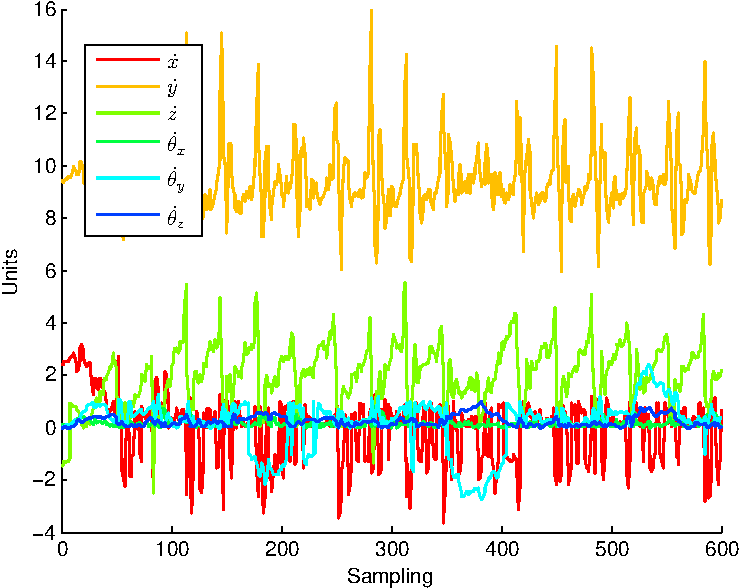
\includegraphics[width=0.25\textwidth]{plots/human_walk-crop.pdf}} 
\subfloat[Human stand to 
seat.]{\label{fig:hb}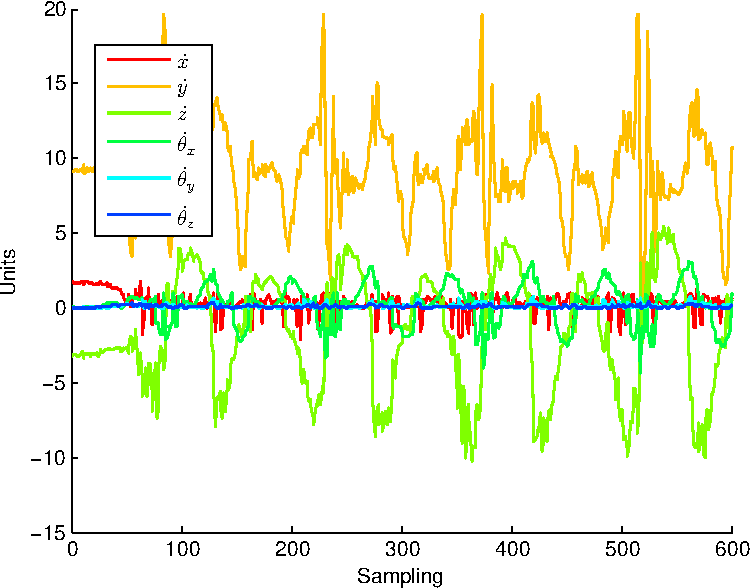
\includegraphics[width=0.25\textwidth]{plots/human_stand-crop.pdf}}
%\subfloat[Human stand to 
%fall.]{\label{fig:hc}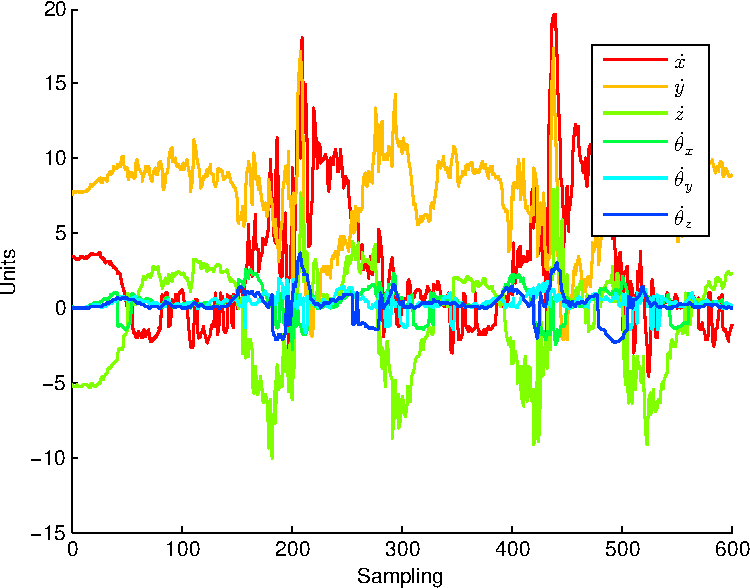
\includegraphics[width=0.32\textwidth]{plots/human_falling-crop.pdf}}
%\\
%\subfloat[Robot walk forward.]{\label{fig:ra}\includegraphics[width=0.32\textwidth]
%{plots/robot_walk_forward-crop.pdf}}
%\subfloat[Robot walk backward.]{\label{fig:rb}\includegraphics[width=0.32\textwidth]
%{plots/robot_walk_backward-crop.pdf}}
%\subfloat[Robot rotate clockwise.]{\label{fig:rc}\includegraphics[width=0.32\textwidth]
%{plots/robot_rotate_cw-crop.pdf}}
%\\
\subfloat[Robot fallen forward.]{\label{fig:rd}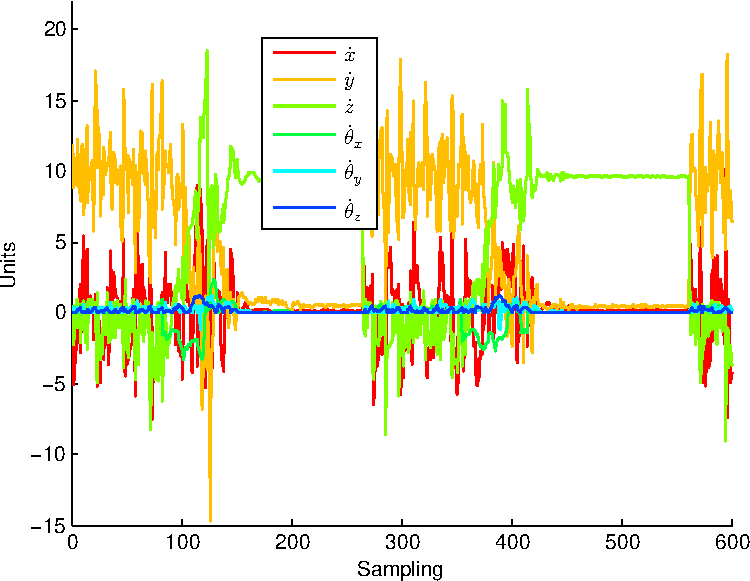
\includegraphics[width=0.25\textwidth]
{plots/robot_fallen_forward-crop.pdf}} 
\subfloat[Robot fallen backward.]{\label{fig:re}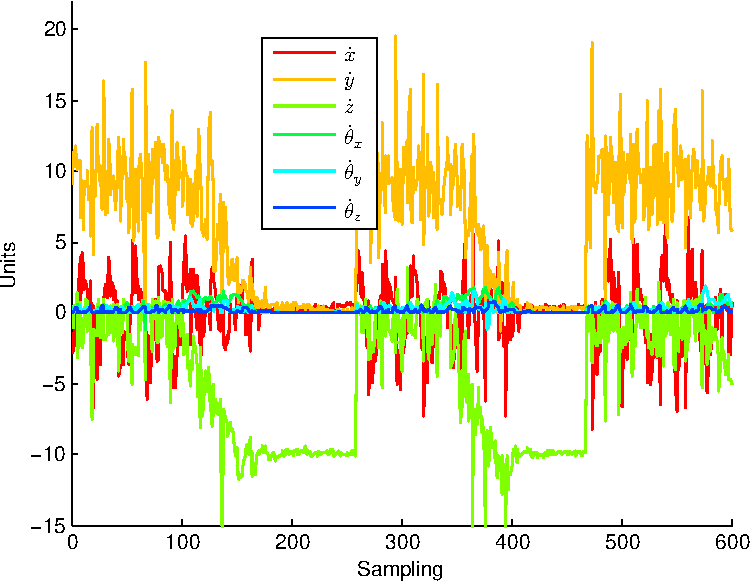
\includegraphics[width=0.25\textwidth]
{plots/robot_fallen_backward-crop.pdf}}
%\subfloat[Robot fallen right.]{\label{fig:rf}\includegraphics[width=0.32\textwidth]
%{plots/robot_fallen_right-crop.pdf}}

\caption{Figures (a)-(b) shows 3-axis accelerometer and 3-axis gyroscope graph for human motions 
walking forward and stand to seat. Figures (c)-(d) shows 3-axis accelerometer and 3-axis gyroscope 
graph for robot's fallen forward and backward motions.}
 \label{fig:anotation-human-robot} 
\end{figure*}
% Figures (d)-(f) shows 3-axis accelerometer and 3-axis gyroscope graph for robot's walk motion. 

We have conducted our experiments on detecting motions (activities) on 
%able-bodied 
humans and humanoid robots (NAO robots). We have used a InvenSense MPU-9150 
motion tracking sensor on the Sensor Hub BoosterPack. 
% 
% The module {\em MPU9150Module} connects to 
% this device and provides the representation {\em MPU9150Representation}. 
% 
We have used 3-axis accelerometer readings, 3-axis gyroscope readings, 3-axis magnetometer readings, 
the quaternion rotation axis of the device, and Euler angles roll, pitch, and yaw.  In order to 
calculate Euler angles, we have used the Direction Cosine Matrix (DCM) algorithm. We have configured 
one device as a remote sensing device, and the other device is configured to receive data from the 
sensing device. The rest of the  section reports our data collection, data processing, learning, 
and prediction results.


\subsection{Activity Annotation}

The annotation for different human and robot motion activities are shown in 
Figure {~\ref{fig:anotation-human-robot}}. 
Accelerometer and gyroscope's $x$, $y$ and $z$ axis are shown for different motions. We can observe 
that an 
actual event takes between 180--250 ms. Figure{~\ref{fig:anotation-human-robot}} (a)-(b) shows the 
activity annotations for human motions (walking forward and sitting down). 
Figure {~\ref{fig:anotation-human-robot}}
(c)-(d) shows activity annotations for the NAO robot. The following section provides the evaluation 
matrices of our experiments. 


\section{Evaluation}
%\subsection{Learning Algorithms}
We have structured this section in a way that we discuss feature extraction, data processing, 
machine learning, and experimental results for both the human and robotic experiments. We have 
tested our hypotheses using  {\em Regularized Logistic Regression} (LLR) and {\em Support 
Vector Machine} (SVM) algorithms. We have used a randomly generated 80\%--20\% partition for 
training and cross-validation on our learning dataset. We have used an independent test set to 
report our results. We have used standard parameter sweeping techniques to find the classifier 
parameters that provide the optimal trade-off between the bias and the variance, while precision, 
recall, and F$_1$-scores have been used to obtain the optimal value. 

\subsection{Feature Extraction}

We  have configured the motion sensor to sample at every  $20ms$, which is equivalent to 50$Hz$ 
sampling rate. In order to 
identify activities: \begin{inparaenum}[1)] \item we have used a window size of $400ms$ (20 
samples); and \item we have allowed 10 samples ($200ms$) to overlap between windows. 
\end{inparaenum} The selection of the window size is based on the observation that a fall event 
takes between $200-300ms$. Thus, a window size of $400ms$ will include both fall event and 
non-fall event data for classification. For each window, we have calculated the running average of 
all 9-axis values. This has produced nine values per window, which has been used as features. We 
also added a bias term to provide additional capacity for the learning algorithms. The  
accelerometer readings are in 3-axis in meter per square second ($m/s^2$), gyroscope readings are 
in 3-axis in radian per square second ($rads/s^2$), and the magnetometer readings are in 3-axis in 
Tesla ($T$). 

As a preprocessing step, the features, except the bias, have been subjected to feature 
standardization. We have independently set each dimension of the sample  to have zero-mean and 
unit-variance. We achieved this by first computing the mean of each dimension across the dataset and 
subtracting this from each dimension. Then each dimension is divided by its standard deviation.
 

\subsection{Experiments with a Human}

We have attached the sensors on the mid-back of the human body as shown in Figure \ref{fig:fb} for  
collecting our datasets. We have collected data for several different  activities. For the studies 
reported here we have used the following datasets:
\begin{inparaenum}[(1)] \item walking forward; \item from standing to sitting down 
and back to standing; and \item from standing to falling and back to standing. \end{inparaenum} 
Example plots for \begin{inparaenum}[1)] \item walking forward; and \item from standing to sitting 
down  \end{inparaenum}  are shown in Figures \ref{fig:ha} and \ref{fig:hb} respectively. 

 \begin{table}[!ht]
\caption{Logistic regression classification for human activities.}
	\label{tab:human-logistic-class}
	\centering
		\begin{tabular} {| l | c | c | c| c|}
		\hline
			{\bf Activity} & {\bf  TP}  &	{\bf TN}  &	{\bf FP} &	{\bf FN} \\ 
\hline
			Walking forward	& 91\%	& 90\%	& 10\%	& 9\% \\ \hline
			Walking backward	& 82\%	& 86\%	& 14\%	& 18\% \\ \hline
			Walking left 	& 86\%	& 86\%	& 14\%	& 14\% \\ \hline
			Walking right 	& 86\%	& 86\%	& 14\%	& 14\% \\ \hline
			Falling forward	& 94\%	& 93\%	& 7\%	& 6\%	 \\ \hline
			Falling Backward	& 84\%	& 88\%	& 12\%	& 16\%	 \\ \hline
			Falling left	& 92\%	& 91\%	& 9\%	& 8\%	 \\ \hline
			Falling Right	& 92\%	& 91\%	& 9\%	& 8\%	 \\ \hline
			Marching	& 91\%	& 90\%	& 10\%	& 9\%	 \\ \hline
			Rotate counter-clockwise	& 91\%	& 89\%	& 11\%	& 9\%	 \\ \hline
			Rotate clockwise	& 92\%	& 89\%	& 11\%	& 8\%	 \\ \hline
		\end{tabular}
\end{table}


\subsubsection{Results:} Table \ref{tab:human-logistic-class} shows the final results for 
LLR classification, where, true positive, true negative, false positive, and false negative are 
abbreviated with TP, TN, FP, and FN respectively. For walking forward on an average, the accuracy is 91\%, 
similarly, for falling forward and marching the accuracies are 94\% and 91\% on an 
average, respectively. We found comparatively low accuracy in walking backward and falling backward. Rotation has accuracy on an average more than 90\%. We also observed that detection of the walking activity is less than other 
activities that we experimented with.  

\begin{table}[!ht]
\caption{SVM classification for human activities.}
	\label{tab:human-svm-class}
	\centering
		
		\begin{tabular} {| l | c | c | c| c|}
		\hline
			{\bf Activity} & {\bf  TP}  &	{\bf TN}  &	{\bf FP} &	{\bf FN} \\ 
\hline
			Walking forward	& 96\%	& 93\%	& 7\%	& 4\% \\ \hline
			Walking backward	& 81\%	& 84\%	& 16\%	& 19\% \\ \hline
			Walking left 	& 89\%	& 90\%	& 10\%	& 11\% \\ \hline
			Walking right 	& 89\%	& 90\%	& 10\%	& 11\% \\ \hline
			Falling forward	& 96\%	& 93\%	& 7\%	& 4\%	 \\ \hline
			Falling Backward	& 84\%	& 87\%	& 13\%	& 16\%	 \\ \hline
			Falling left	& 93\%	& 93\%	& 7\%	& 7\%	 \\ \hline
			Falling Right	& 92\%	& 93\%	& 7\%	& 8\%	 \\ \hline
			Marching	& 95\%	& 93\%	& 7\%	& 5\%	 \\ \hline
			Rotate counter-clockwise	& 93\%	& 91\%	& 9\%	& 7\%	 \\ \hline
			Rotate clockwise	& 94\%	& 91\%	& 9\%	& 6\%	 \\ \hline
		\end{tabular}
\end{table}


The results for SVM classifier is summarized in Table \ref{tab:human-svm-class}. On an average, 
accuracy for each type of activity is higher than LLR classifier with on an average 96\% for 
walking, 95\% for marching, and 96\% for falling forward. Both type of rotations have little higher accuracy over LLR. As a consequence, SVM classifier has less false positives and false negative compared to LLR.  Our experiments reveal that the SVM classifier performs better than the logistic regression classifier. However, due to memory and 
computational restrictions on the embedded devices, we have found that the logistic 
regression classifier is a better choice.  Our feature vector consists of the mean normalized sensor 
reading and a bias term. We plan to combine and prune features to improve the classification 
accuracy for future work.  


\subsection{Experiments with a NAO Robot}
 

\begin{figure*}[!ht]
  \centering
  \subfloat[Marching in place.]{\label{fig:tsnedataset_1}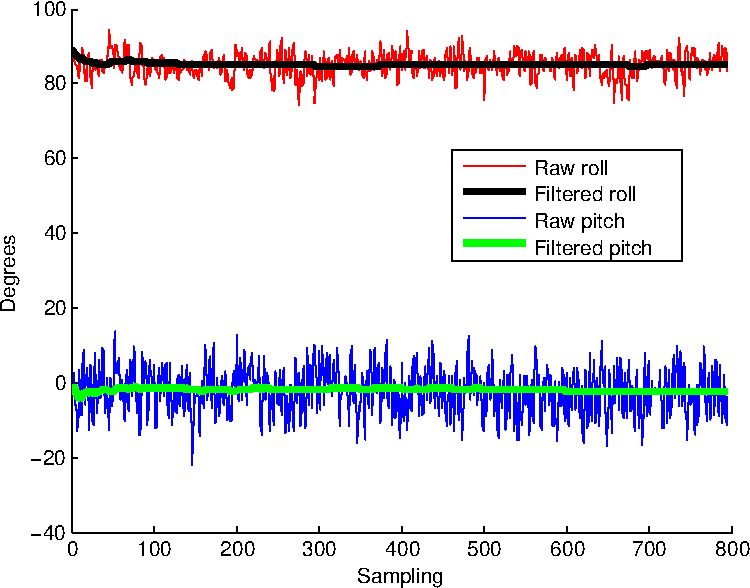
\includegraphics[width=0.25\textwidth]
       {plot1-crop}} 
  \subfloat[Walking backward.]{\label{fig:tsnedataset_9}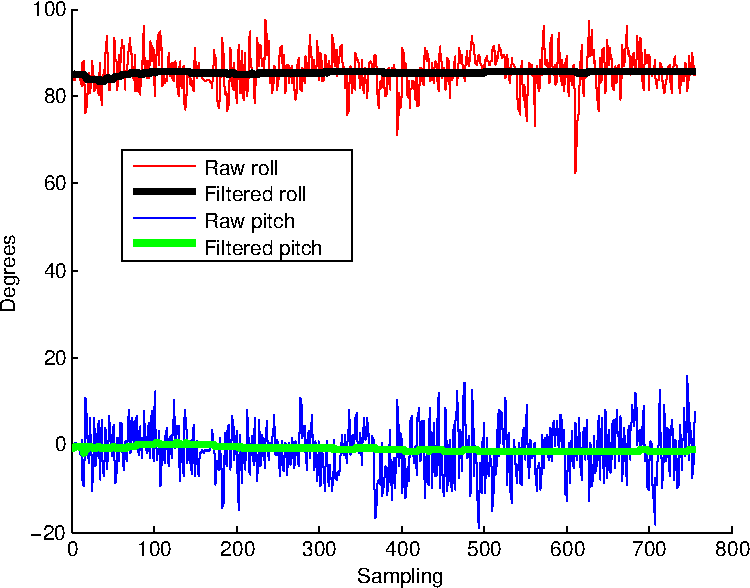
\includegraphics[width=0.25\textwidth]
       {plot5-crop}}
%  \subfloat[Rotating clockwise.]{\label{fig:tsnedataset_7}\includegraphics[width=0.25\textwidth]
%       {plot2-crop}}
%  \subfloat[Left side-way walk.]{\label{fig:tsnedataset_10}\includegraphics[width=0.25\textwidth]
%       {plot6-crop}}
%       \\
  \subfloat[Falling forward.]{\label{fig:tsnedataset_11}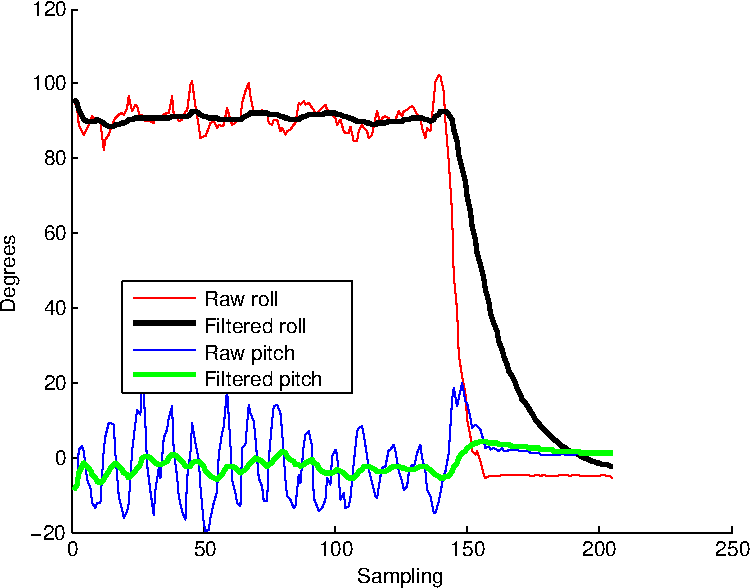
\includegraphics[width=0.25\textwidth]
       {plot1_fallen-crop}}
  \subfloat[Falling backward.]{\label{fig:tsnedataset_12}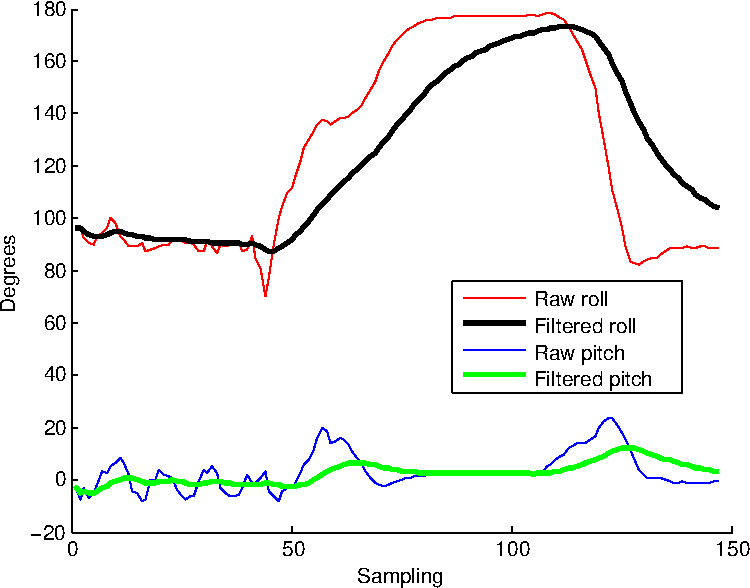
\includegraphics[width=0.25\textwidth]
       {plot2_fallen-crop}}
%  \subfloat[Falling to left side.]{\label{fig:tsnedataset_13}\includegraphics[width=0.25\textwidth]
%       {plot3_fallen-crop}}
%  \subfloat[Falling to right
%side.]{\label{fig:tsnedataset_14}\includegraphics[width=0.25\textwidth]
%       {plot4_fallen-crop}}      
  \caption{Figures (a)-(b) show the roll and pitch angles (raw and filtered) for normal 
behaviors marching in place and walking backward. Figures (c)-(f) show the raw and filtered roll 
and pitch angles for fallen forward and backwards states of NAO humanoid robot.}
  \label{fig:normalFallenBehavior}

\end{figure*}


Our NAO robots have an omni-directional walking engine.  
Walking motions are regulated by linear velocities $\dot{x}_v$ and $\dot{y}_v$, and an 
angular velocity $\dot{\theta}_v$ as input parameters. Depending on these
values we can let the robot walk (forward, backward, and side-ways) and rotate (clockwise and
counter-clockwise) with different speeds. In this study, we have considered \begin{inparaenum}[(1)]
\item marching ($\dot{x}_v = 0 , \dot{y}_v = 0, \dot{\theta}_v = 0$); \item walking  
forward/backward ($\dot{x}_v = \pm200
, \dot{y}_v = 0, \dot{\theta}_v = 0$);  \item walking side-ways ($\dot{x}_v = 0, \dot{y}_v = 
\pm200, \dot{\theta}_v = 0$); and  \item rotating clockwise/counter-clockwise
($\dot{x}_v = 0 , \dot{y}_v = 0, \dot{\theta}_v = \pm 0.5$) \end{inparaenum} as {\em normal states}, 
while all the other activities are classified as {\em fallen states}. 

\begin{table}[!ht]
\caption{Logistic regression classification for robot activities.}
	\label{tab:robot-logistic-class}
	\centering
		\begin{tabular} {| l | c | c | c| c|}
		\hline
			{\bf Activity} & {\bf  TP}  &	{\bf TN}  &	{\bf FP} &	{\bf FN} \\ 
\hline
			Walking forward	& 91\%	& 90\%	& 10\%	& 9\% \\ \hline
			Walking backward	& 90\%	& 90\%	& 10\%	& 10\% \\ \hline
			Walking left 	& 92\%	& 90\%	& 10\%	& 8\% \\ \hline
			Walking right 	& 89\%	& 90\%	& 10\%	& 11\% \\ \hline
			Falling forward	& 94\%	& 93\%	& 7\%	& 6\%	 \\ \hline
			Falling Backward	& 94\%	& 93\%	& 7\%	& 6\%	 \\ \hline
			Falling left	& 95\%	& 93\%	& 7\%	& 5\%	 \\ \hline
			Falling Right	& 94\%	& 93\%	& 7\%	& 6\%	 \\ \hline
			Marching	& 91\%	& 89\%	& 11\%	& 9\%	 \\ \hline
			Rotate counter-clockwise	& 97\%	& 92\%	& 8\%	& 3\%	 \\ \hline
			Rotate clockwise	& 98\%	& 92\%	& 8\%	& 2\%	 \\ \hline
		\end{tabular}
\end{table}



We have attached the sensors on the back of the NAO humanoid robot as shown in Figure \ref{fig:fc} 
and used the following protocol to collect the datasets. First, we set the velocity 
parameters and activate the walking engine of the robot. Then, we collect the motion data 
transmitted by the wireless device attached at the back of the robot. Finally, we marked the start 
point of the sample stream and collect data approximately for a minute and marked the end of the 
sample stream. This is an episode of a normal  or a fallen state. We repeat the about described 
protocol for collecting multiple episodes to obtain our learning ensemble. To collect samples for 
fallen states, we have configured the walking engine to marching activity. Then, we safely pushed 
the robot to different directions to inducing the fallen state. Similarly, we marked the sample 
streams to generate several episodes for the learning ensemble.    

\begin{table}[!ht]
\caption{SVM classification for robot activities.}
	\label{tab:robot-svm-class}
	\centering
		\begin{tabular} {| l | c | c | c | c | }
		\hline
			{\bf Activity} & {\bf  TP}  &	{\bf TN}  &	{\bf FP} &	{\bf FN} \\ 
\hline
			Walking forward	& 93\%	& 91\%	& 9\%	& 7\% \\ \hline
			Walking backward	& 93\%	& 91\%	& 9\%	& 7\% \\ \hline
			Walking left	& 94\%	& 90\%	& 10\%	& 6\% \\ \hline
			Walking right	& 90\%	& 91\%	& 9\%	& 10\% \\ \hline
			Falling forward	& 98\%	& 93\%	& 7\%	& 2\%	 \\ \hline
			Falling backward	& 98\%	& 93\%	& 7\%	& 2\%	 \\ \hline
			Falling left	& 99\%	& 94\%	& 6\%	& 1\%	 \\ \hline
			Falling right	& 98\%	& 93\%	& 7\%	& 2\%	 \\ \hline
			Marching	& 90\%	& 91\%	& 11\%	& 10\%	 \\ \hline
			Rotate counter-clockwise	& 97\%	& 93\%	& 7\%	& 3\%	 \\ \hline
			Rotate clockwise	& 96\%	& 93\%	& 7\%	& 4\%	 \\ \hline
		\end{tabular}
\end{table}


\subsubsection{Results:}

The results for LLR and SVM classifiers are summarized in Tables \ref{tab:robot-logistic-class} and 
\ref{tab:robot-svm-class}. The results are similar to identification of human activities, for 
conserving space, we omit detail discussion of the results. It is worthwhile to note that the SVM 
 identified events more accurately than LLR as observed for human activities.  

% Even though the thresholding method successfully distinguished between normal and fallen states, 
%we 
% were 
% unable to detect states within normal activities, i.e., walking forward to walking backward etc.. 
% Therefore, similar to the previous experiments, we have used logistic regression and SVM 
% classifiers to identify different activities. We have followed the same protocols as mentioned in 
% the previous section to generate features, learning, and prediction. Table 
% \ref{tab:robot-logistic-class} shows the results for the logistic regression classifier while 
% Table \ref{tab:robot-svm-class} shows the results for the SVM classifier.    



% We conclude that the classification methods are able to predict activities within normal states 
% as well as fallen states. Similar to the previous experiments with a human, the SVM classifier 
% performs 
% better that the logistic regression classifier, though, during operation, we prefer the logistic 
% regression classifier. The range of motion of the NAO robot is comparatively constrained compared to 
% a 
% human. Therefore, we can only conduct primary activities as described in this section. We have not 
% conducted experiments on activities such as \textit{standing to sitting down}. When determining the 
% results, we 
% have sampled the motion device data at the rate 50$Hz$. During operation, if the 
% thresholding method is used, we can use the same thresholds with higher sampling rates. The second 
% method requires learning for different sampling rates.

Even though the above learning methods provide accurate results, there are microcontrollers with 
very limited computational and memory capacities. In such devices, it is better to use less memory 
expensive methods such as Kalman filtering, which is reported in the next section.

\subsubsection{Kalman Filtering:}

We have designed a thresholding base activity predictor in these experiments. Using the the same 
datasets, we have calculated the roll, pitch, and yaw angles  using the DCM algorithm. In order to 
achieve an effective threshold-based decision making, we have filtered the roll, pitch, and
yaw values using a Kalman filter \cite{Welch:1995:IKF:897831}. Figures 
\ref{fig:normalFallenBehavior} ((a)--(b)) show the raw and the filtered values of the raw and the 
pitch values for marching and walk backward. The other activities show similar plots (we have 
refrained from plotting them due to space constraints). 

The thresholding method suggests that, if the filtered roll values are within the range $[90\pm15]$ 
(degrees) and the filtered pitch values are within the rage $[0\pm15]$ (degrees), then with 100\% 
accuracy, the NAO  robot will be in a normal state. Otherwise, we can safely assume that the robot 
is in a fallen state. Figures \ref{fig:normalFallenBehavior} ((c)--(d)) show the roll and pitch 
angles (raw and filtered) for a typical fallen robot. If the filtered roll value is less that 60 
degrees, we can safely assume that the robot is falling forward. If the filtered roll values is 
more than 100$^{\circ}$ we can assume that the robot is falling backward. To detect the events 
falling to the left and right, we have used the filtered pitch values. If the filtered pitch value 
is less than -50$^{\circ}$, we can assume that the robot is falling to the left side, while if the 
filtered pitch values is more than 50$^{\circ}$, we can assume that the robot is falling to the right 
side. With these thresholds for a separate test cases, the thresholding method has detected fallen 
state with 100\% accuracy. 

Even though the thresholding method successfully distinguished between normal and fallen 
activities, it was unable to detect states within the normal activities, i.e., walking forward 
to walking backward so on. This one of the limitation of using thresholding methods, which has 
been overcome by the learning methods.  We use Kalman filter in this experiments because of its 
efficacy and the choice of the filter is entirely arbitrary depending on the computational 
resources of the microcontroller.  


\section{Conclusion and Future Work}

It is known that while humans and biped humanoid robots perform normal activities such as jogging, 
running and so on, an abnormal event such as a fall may occur. These events may cause injuries 
 to the humans or robots. 
%  In order to avoid 
%  damages to biped humanoid robots, machine learning can be used to predict potential falls before 
%  such events occur. 
  Using the prediction information, corrective measures can be engaged to avoid 
 many fall activities. Similarly, for humans, after  a fall activity is identified, rescue services 
 can be called upon. We have reported a wireless sensing device that have assembled using 
off-the-shelf hardware components. Using two devices, we have created a sensor network for 
collecting motion data from humans and biped humanoid robots. The sensing devices were connected to 
the back of the subjects and the data collecting device was connected to a laptop which archived 
the data. We have used two machine learning algorithms and a thresholding methods to 
identify both normal and abnormal activities within 91\%--100\% accuracy. Comparing the encouraging 
experimental results we achieved, our future work will be to use multiple sensing devices to create 
a sensor network to detect complex activities with higher sampling rates.  

\bibliographystyle{aaai}
\bibliography{references}

\end{sloppy}
\end{document}
